% !TEX root = ../main.tex
\section{Spellcasting Rules} \label{sec::spellcastingrules}
\subsection*{Spellcasting Doctrines}
    There exist five spellcasting doctrines in Yuadrem, each related to a tide.
    Many schools belong to each doctrine, but all are related at heart.

    In general, casting a spell requires certain conditions to be met.
    These conditions depend on the spell itself, but can be categorized by the spellcasting doctrine to which they belong.
    Each doctrine and its method for casting spells is detailed in this section.

    \subsubsection{Sympathy}
        Sympathists manifests effects on the world via sympathetic links.
        These links can be of three natures: heat, electric, and similarity.

        \subparagraph{Heat Link}
        (see page \pageref{medium::ember}).
        Sympathy spellcasters can quickly produce great surges of energy around them, but these are useless without a spark to ignite them.
        Heat links are floating embers which act as these sparks.

        \subparagraph{Electric Link}
        (see page \pageref{medium::charge}).
        In contrast with fire, sympathists don't require a spark to manifest energy in its most pure form: electricity.
        Nonetheless, without a charge to guide lightning, it just takes the shortest route towards the ground.
        Sympathists use electric links to apply these charges to creatures and objects around them, enabling them to direct lightning at foes and allies alike.

        \subparagraph{Similarity Link}
        (see page \pageref{medium::tether}).
        Unlike other sympathetic mediums, similarity links connect creatures and objects to exchange properties between them.
        A sympathist can tether these links to, for example, increase the weight of a creature, change its form, levitate it, etc.

        When you take the spellcaster feat and choose the sympathy doctrine, choose two of these mediums.
        When you do so, you learn the associated spells, and can start learning any of the spells that require these links to work.
        In addition, you learn one additional link, which is related to your school.
        Schools and their special links are detailed in the sympathy section (see page \pageref{sec::sympathy}).

    % \subsubsection{Sigaldry}
        % \textbf{TODO}.

    % \subsubsection{Alchemy}
        % \textbf{TODO}.

    % \subsubsection{Thaumaturgy}
        % \textbf{TODO}.

    % \subsubsection{Eldremry}
        % \textbf{TODO}.

\subsection*{Spellcasting Ability}
    When you take the spellcaster feat, you decide a spellcasting ability, which can be Intelligence, Wisdom, or Charisma.
    This choice reflects your medium for casting spells: Conceptualization for Intelligence, volition for Wisdom, and empathy for Charisma.

    You use this ability score whenever a spell refers to your spellcasting ability.
    In addition, you use its modifier when setting the saving throw DC for a spell you cast and when making an attack roll with one.

    \textbf{Spell save DC} = 8 + your spellcasting proficiency bonus + your chosen ability modifier

    \textbf{Spell attack modifier} = your spellcasting proficiency bonus + your chosen ability modifier

    After taking the spellcaster feat, your spellcasting proficiency bonus is +2.
    You can increase this modifier further by taking the \textbf{Avid Caster} feat (see page \pageref{feat::avidcaster}).

\subsection*{Known Spells}
    As a user of magic, you know a number of spells which you can use in any scenario you find appropiate.
    The maximum number of spells you can have prepared at a time is equal to your spellcasting ability modifier + half your level (rounded down).
    If you add a new spell when you already have the maximum number of spells prepared, you forget one spell of your choice.
    To keep these spells available, you can use a spellbook (see page \pageref{item::spellbook}).

    When you take the \textbf{Spellcaster} feat (page \pageref{feat::spellcaster}), you gain access to three mediums and two spells.
    Two of the mediums and one spell are of your choice within your chosen doctrine, and the other medium and spell comes from the spellcasting school of your choice.
    The spell associated to your school does not count towards your number of known spells.

    All spells come in two levels.
    When you take the \textbf{Spellcaster} feat you only gain access to the first level of these spells.
    By taking the \textbf{Upgraded Spellcasting} major character advancement (see page \pageref{mca::upgradedspellcasting}), showing your commitment to your school, you gain access to the second level of spells.

    You can learn one new spell as part of a long rest.
    This spell must belong to a spellcasting doctrine available to you.

\subsection*{Spell Points}
    Your character uses spell points to fuel spells.
    Each spell has a point cost based on its strength, which is detailed in the spell's description.
    Mediums don't require spell points to be cast.
    You recover all spent spell points after a short rest.

    The number of spell points you have to spend is based on your level, as shown in the spellcasting ability table.
    In addition, you can gain access to more spell points by taking the \textbf{Upgraded Spellcasting} major character advancement.

    \begin{DndTable}[width=\linewidth, header=Spellcasting Ability]{lllll}
        \textbf{Level} &  \textbf{Spell Points} & \hspace{0.5cm} & \textbf{Level} & \textbf{Spell Points} \\
         1st &     2 &  & 11th &    36 \\
         2nd &     3 &  & 12th &    38 \\
         3rd &     7 &  & 13th &    41 \\
         4th &     8 &  & 14th &    44 \\
         5th &    13 &  & 15th &    47 \\
         6th &    16 &  & 16th &    50 \\
         7th &    19 &  & 17th &    53 \\
         8th &    22 &  & 18th &    57 \\
         9th &    28 &  & 19th &    61 \\
        10th &    32 &  & 20th &    66
    \end{DndTable}

    \thispagestyle{empty} % Remove footer so that it doesn't clash with the image.
    \begin{tikzpicture}[remember picture,overlay]
        \node[anchor=south, yshift=-0.10cm] at (current page.south) {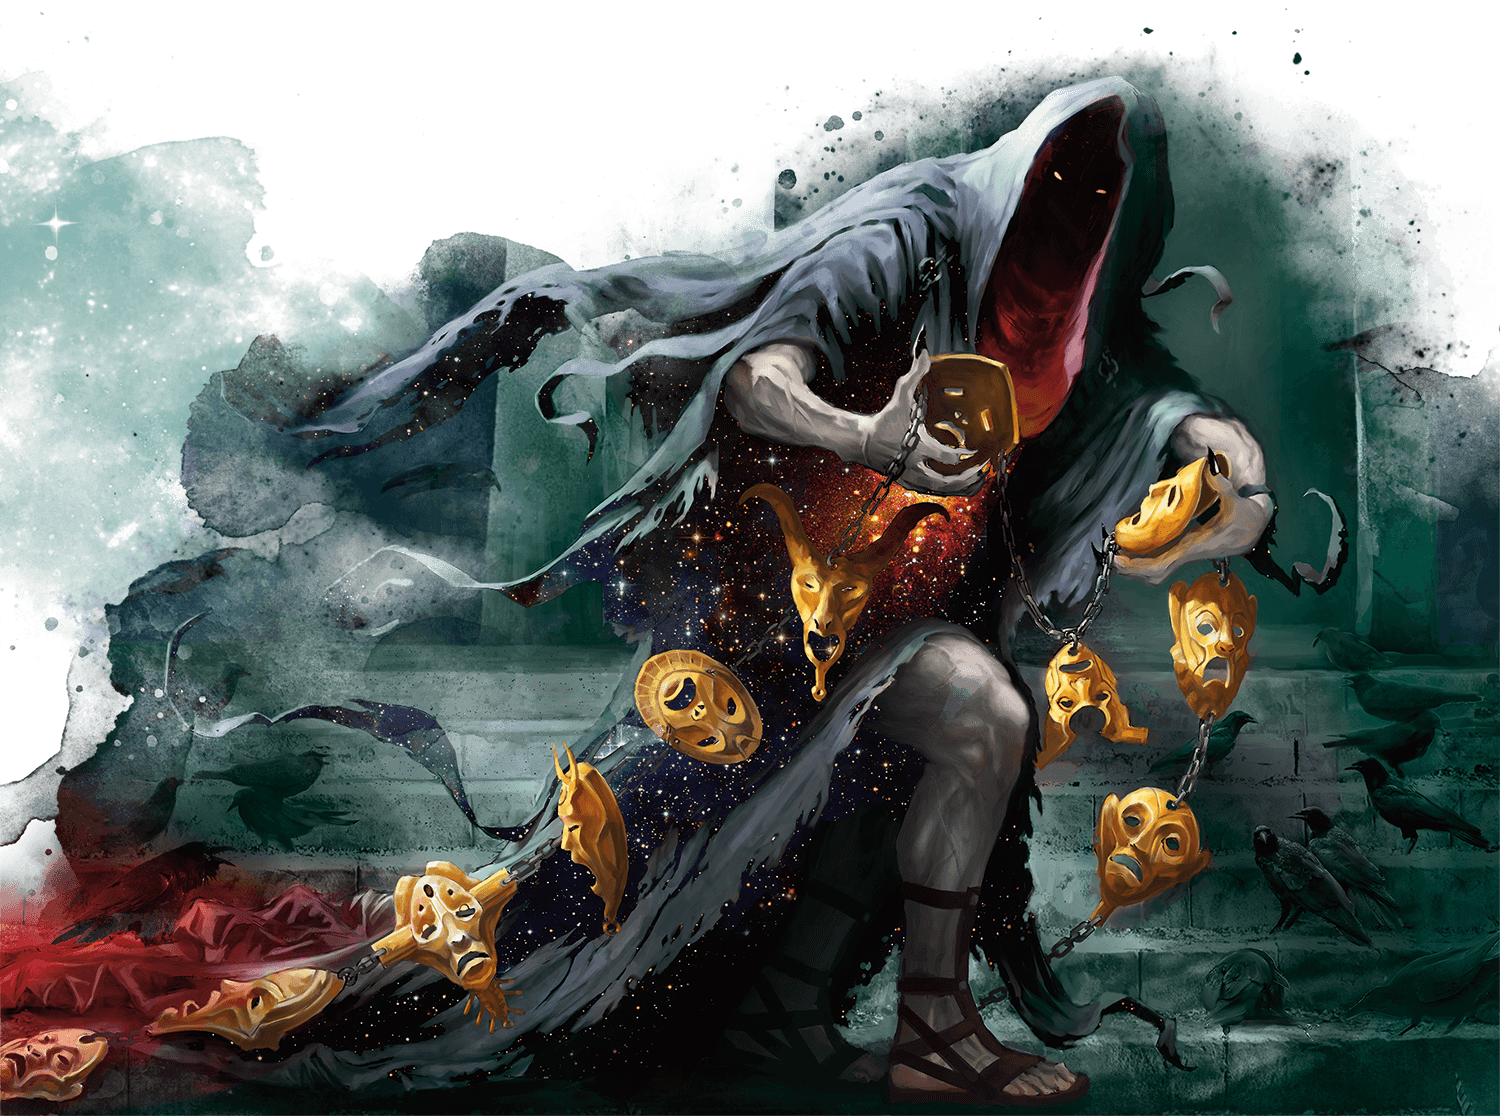
\includegraphics[width=\pdfpagewidth]{08spellcasting/img/10erebos.png}};
    \end{tikzpicture}

\newpage
% NOTE. I will probably end up filling this space (and more!) when I add descriptions for the other spellcasting doctrines.

~\newpage
